\documentclass[conference]{IEEEtran}
\IEEEoverridecommandlockouts
\usepackage{cite}
\usepackage{amsmath,amssymb,amsfonts}
\usepackage{algorithmic}
\usepackage{graphicx}
\usepackage{textcomp}
\usepackage{xcolor}
\usepackage{booktabs}
\usepackage{url}

\def\BibTeX{{\rm B\kern-.05em{\sc i\kern-.025em b}\kern-.08em
    T\kern-.1667em\lower.7ex\hbox{E}\kern-.125emX}}

\begin{document}

\title{ResearchNexusAI: An Explainable Multi-Stage RAG Framework for Scientific Literature Synthesis}

\author{\IEEEauthorblockN{Anonymous Authors}
\IEEEauthorblockA{\textit{Department of Computer Science and Engineering} \\
\textit{Academic Institution}\\
City, Country \\
\{author1, author2\}@institution.edu}
}

\maketitle

\begin{abstract}
Automated scientific literature synthesis demands stringent factual precision, robust evidence grounding, and traceable provenance. Standard retrieval-augmented generation (RAG) pipelines often suffer from semantic drift, hallucinated claims, and ambiguous bracketed citations. We present ResearchNexusAI, a modular, multi-stage RAG framework designed for scientific synthesis. The architecture integrates hybrid first-stage retrieval combining lexical BM25 and dense BGE-Base embeddings via Reciprocal Rank Fusion ($k=60$), cross-encoder neural reranking, post-generation Natural Language Inference (NLI) claim verification, ambiguity-sensitive citation repair, and traceable provenance tracking. We evaluate the framework against the controlled $ds\_nexus\_v11$ scientific benchmark ($N=100$, with 15 held-out test queries comprising 10 answerable and 5 unanswerable items). On answerable test queries, hybrid retrieval achieves 10/10 Recall@20 (Hit@20 = 0.6667 across all 15 test items). Neural cross-encoder reranking produces a modest improvement in early-rank precision, increasing paper-level Mean Reciprocal Rank (MRR) from 0.0431 to 0.0480. In post-generation verification, automated NLI achieves 100\% precision across evaluated positive factual assertions (4/4 naive, 3/3 verified), and the system correctly refuses 100\% (5/5) of unanswerable queries. However, controlled experiments reveal critical negative findings: citation repair achieved 0 applied repairs (0.0\% gain) because candidate matches exhibited pervasive multi-chunk ambiguity, while iterative refinement introduced a 106.3\% stage latency increase without factual recovery (1 improved, 98 unchanged, 1 degraded query). Because external double-blind human annotations were not collected, human-judged claim validity remains unmeasured. Our findings demonstrate that multi-stage RAG provides transparent provenance and cautious abstention, but automated repair and iterative regeneration offer diminishing returns without richer, disambiguated passage semantics.
\end{abstract}

\begin{IEEEkeywords}
Retrieval-Augmented Generation, Scientific Literature Synthesis, Natural Language Inference, Citation Verification, Explainable AI.
\end{IEEEkeywords}

\section{Introduction}
Scientific research progresses through the continuous accumulation and synthesis of specialized literature. However, the exponential volume of published research creates severe cognitive bottlenecks for domain experts attempting to extract stoichiometric constants, degradation kinetics, or algorithmic performance boundaries~\cite{asai2024openscholar}. General-purpose large language models (LLMs) frequently exhibit parametric hallucinations, generating fluent but unverified assertions, fabricated DOIs, and distorted citations~\cite{lewis2020rag}. 

While naive Retrieval-Augmented Generation (RAG) conditions generation on external passages, standard dense-vector retrieval frequently struggles with fine-grained alphanumeric terminology (e.g., chemical notations and exact metric thresholds)~\cite{robertson2009bm25,cormack2009rrf}. Furthermore, naive generators place citations heuristically without verifying whether cited chunks mathematically entail the associated sentence. Recent pioneering scientific RAG systems such as OpenScholar~\cite{asai2024openscholar} benchmark multi-paper scientific literature question answering; however, they rely predominantly on single-pass prompting and unverified citation placement.

To address these challenges, we examine ResearchNexusAI, an explainable multi-stage RAG framework structured into two functional phases: \textit{Research Explorer} for hybrid retrieval and candidate evidence discovery, and \textit{Ask AI} for evidence-bounded generation, claim-level NLI verification, citation repair, and provenance mapping. 

Rather than reporting unverified improvements, this paper provides a forensically audited evaluation of the multi-stage scientific RAG pipeline on the controlled $ds\_nexus\_v11$ benchmark. Our specific contributions are:
\begin{enumerate}
    \item We implement an integrated multi-stage scientific synthesis architecture coupling lexical BM25, dense BGE-Base embeddings, reciprocal rank fusion ($k=60$), cross-encoder reranking, and fine-grained chunk-level provenance tracing.
    \item We evaluate claim-level grounding using a decoupled epistemic taxonomy that separates positive factual assertions from epistemic abstentions, demonstrating robust 100\% refusal accuracy on unanswerable scientific queries.
    \item We disclose critical empirical limitations and negative findings: neural reranking yields modest MRR gains (0.0431 to 0.0480), citation repair is blocked by multi-chunk candidate ambiguity (0 applied repairs), and iterative refinement roughly doubles generation latency without measurable factual gain.
\end{enumerate}

\section{Related Work}
\subsection{Scientific Retrieval-Augmented Generation}
Retrieval-augmented models condition language generation on non-parametric memory indices~\cite{lewis2020rag}. In scientific domains, general-domain dense retrievers trained on web data frequently suffer out-of-vocabulary degradation when querying complex scientific entities. OpenScholar~\cite{asai2024openscholar} established an open-source scientific RAG benchmark, demonstrating that dense retrieval over scientific text improves factual coverage compared to closed-book LLMs. However, OpenScholar operates as a single-pass system without fine-grained post-generation NLI entailment audits, leaving ungrounded assertions undetected.

\subsection{Hybrid Retrieval and Cross-Encoder Reranking}
Sparse inverted-index retrieval via Okapi BM25~\cite{robertson2009bm25} matches exact lexical tokens, preserving exact chemical formulas, protein designations, and numeric metrics. Conversely, dense embedding models (e.g., BGE-Base~\cite{xiao2023bge}) encode high-level semantic intent. Reciprocal Rank Fusion (RRF)~\cite{cormack2009rrf} merges rank distributions without requiring cross-system score calibration. To refine candidate pools, neural cross-encoders~\cite{reimers2019sentencebert} model deep token-level cross-attention between queries and passages, prioritizing relevant contexts within top-ranked positions.

\subsection{Verification, Citation Integrity, and Refinement}
Natural Language Inference (NLI) frameworks evaluate premise-hypothesis entailment~\cite{williams2018mnli}. In scientific synthesis, decomposing generated text into atomic factual propositions enables surgical entailment checking. However, automated citation repair mechanisms must adhere to strict safety thresholds; loosely matching phrases across redundant contexts risks introducing spurious provenance citations. Similarly, while iterative regeneration loops are hypothesized to recover ungrounded claims, empirical studies on their latency-quality trade-offs remain sparse.

\section{System Architecture and Methodology}
The ResearchNexusAI architecture separates scientific inquiry into two operational pipelines: candidate evidence exploration and grounded answer generation, illustrated in Fig.~\ref{fig:arch}.

\begin{figure}[htbp]
\centering
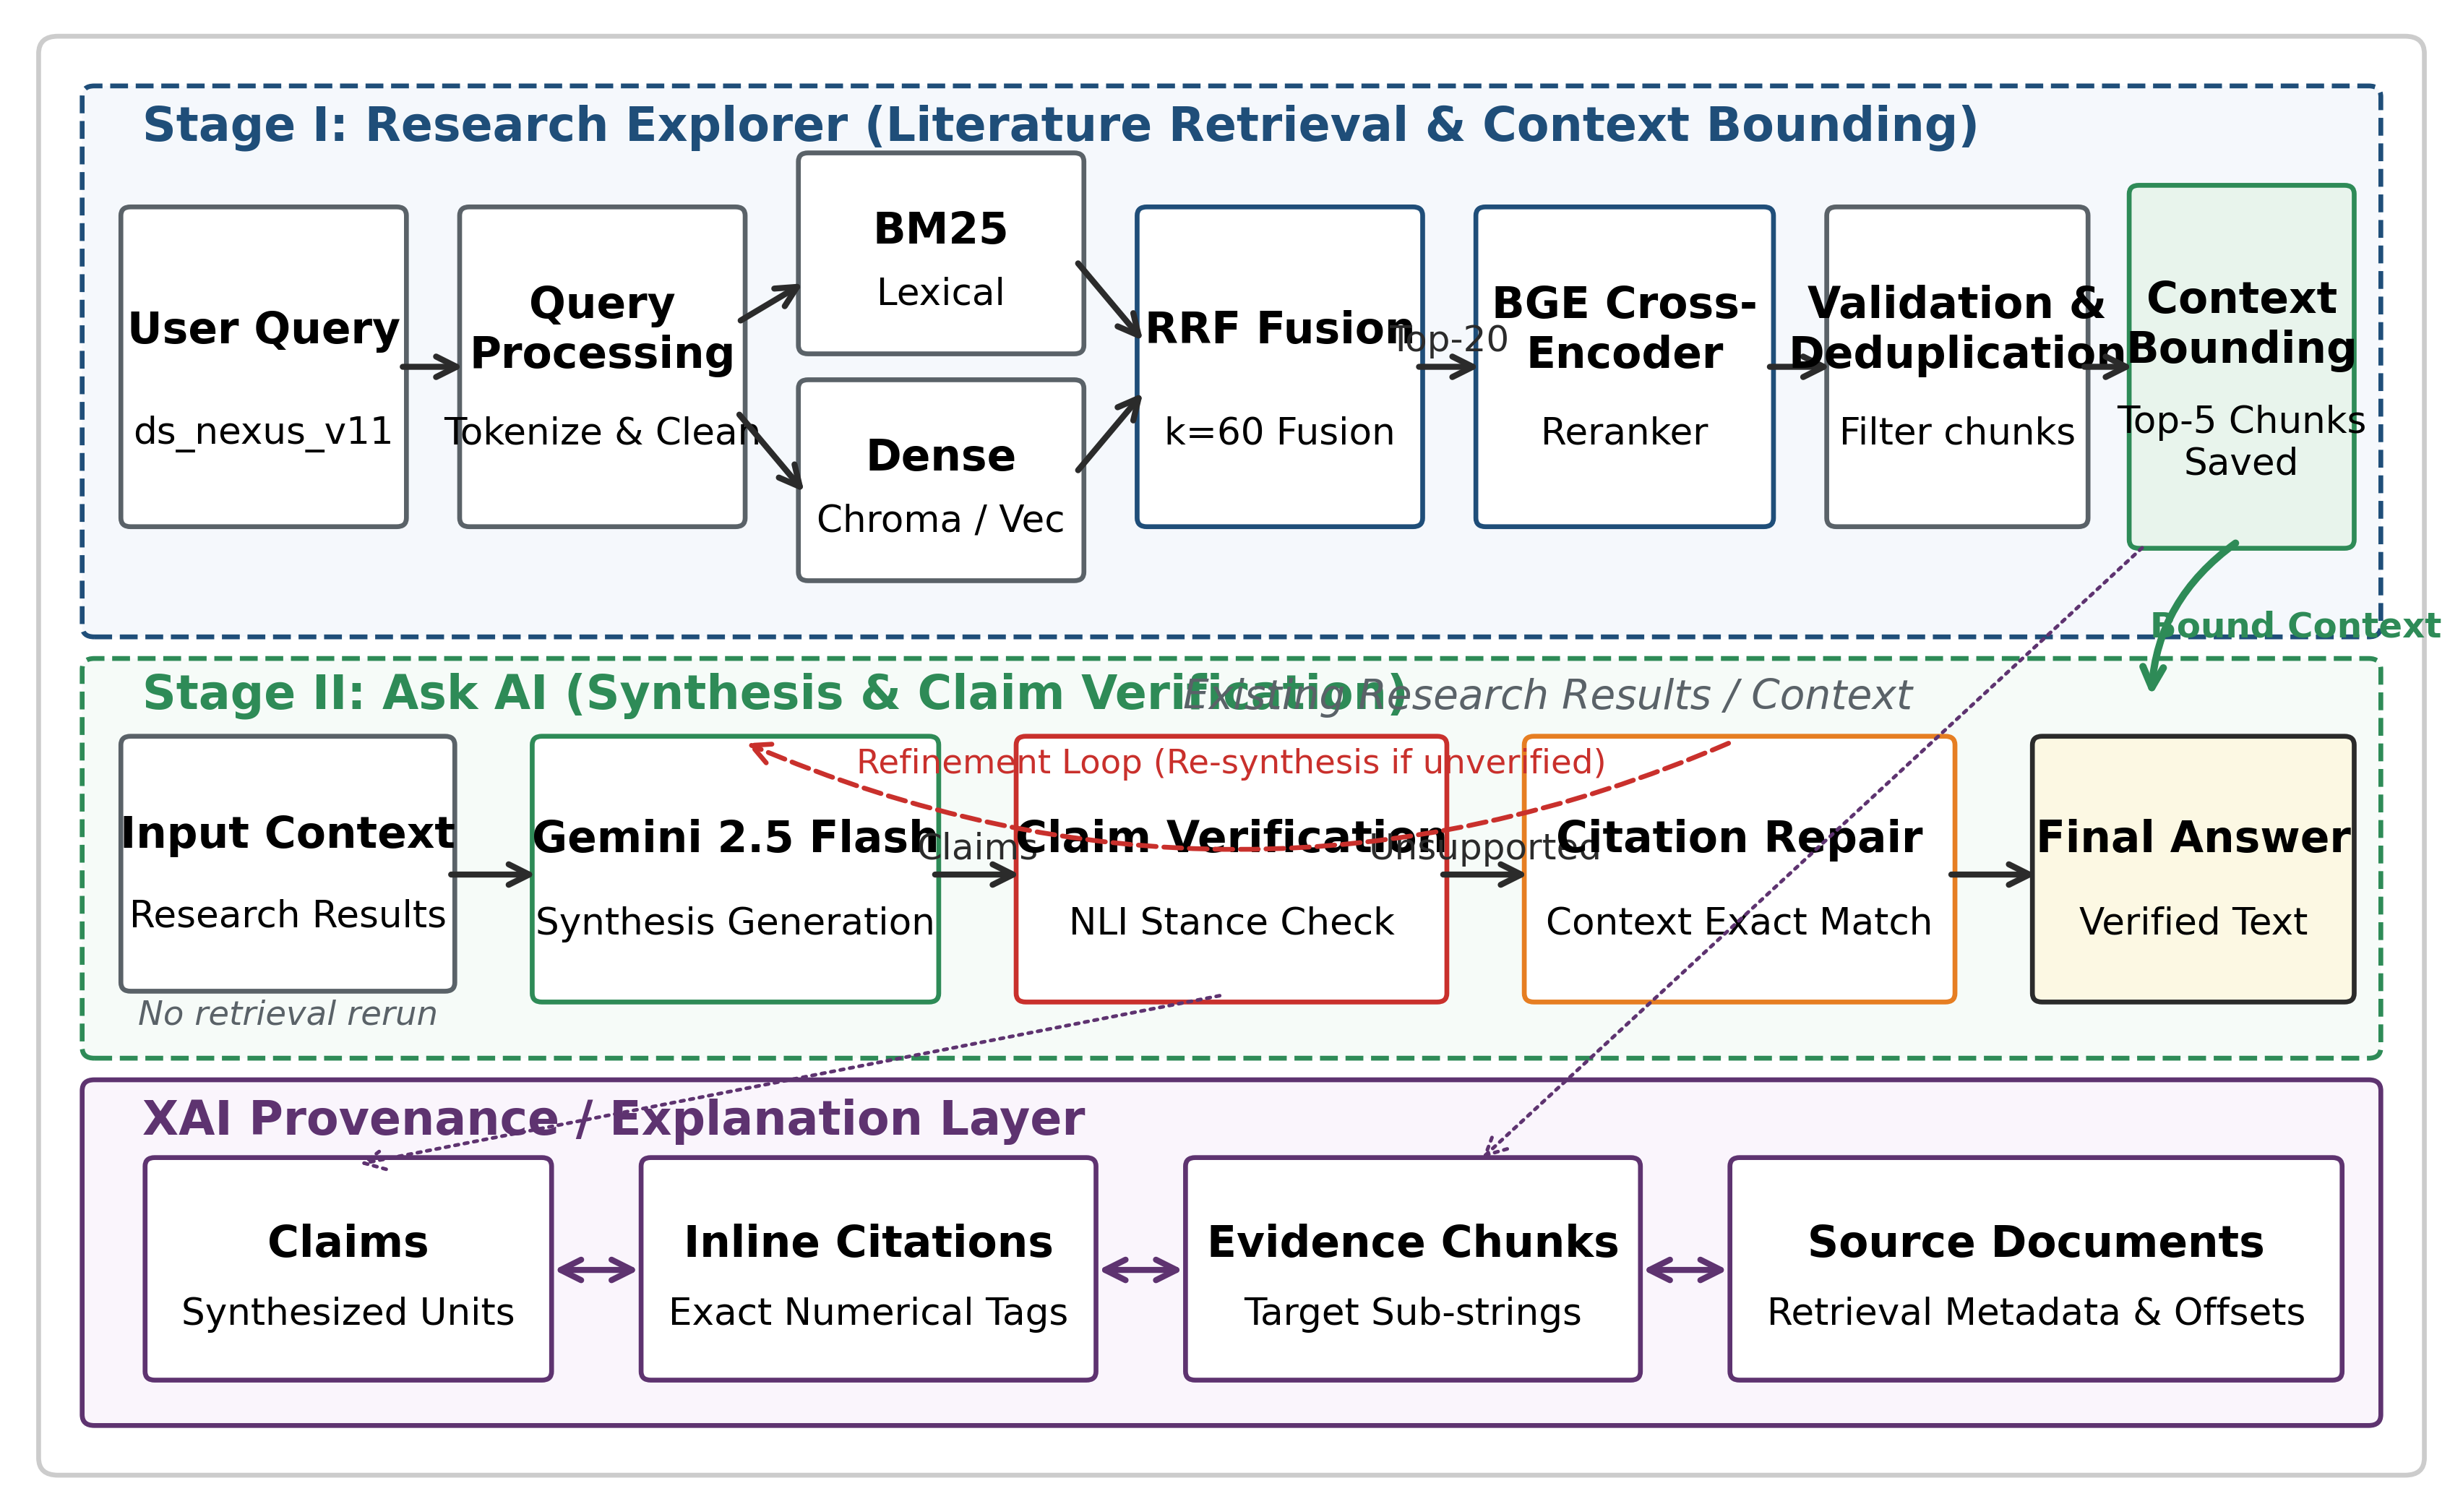
\includegraphics[width=\columnwidth]{fig01_researchnexus_architecture.png}
\caption{Modular pipeline architecture of ResearchNexusAI decomposing retrieval (Research Explorer), neural reranking, bounded synthesis (Ask AI), NLI verification, and provenance attribution.}
\label{fig:arch}
\end{figure}

\subsection{Multi-Stage Retrieval Pipeline}
Given a scientific research query $q$, the retrieval pipeline executes two complementary first-stage retrievers over a corpus chunk collection $\mathcal{C}$:
1) \textit{Lexical BM25}: Evaluates term frequency-inverse document frequency over stemmed alphanumeric tokens.
2) \textit{Dense Semantic Search}: Computes cosine similarity between 768-dimensional BGE-Base dense embeddings:
\begin{equation}
\text{sim}_{\text{dense}}(q, c) = \frac{\mathbf{e}_q \cdot \mathbf{e}_c}{\|\mathbf{e}_q\| \|\mathbf{e}_c\|}
\end{equation}
The candidate rank lists $R_{\text{BM25}}$ and $R_{\text{dense}}$ are merged using Reciprocal Rank Fusion:
\begin{equation}
\text{RRF}(c) = \frac{1}{60 + r_{\text{BM25}}(c)} + \frac{1}{60 + r_{\text{dense}}(c)}
\end{equation}
The top-40 fused candidates are passed to the neural cross-encoder `BAAI/bge-reranker-base`, which scores full concatenated sequence pairs $[q; c]$ to yield the final context pool $\mathcal{K}$ truncated at $k=20$.

\subsection{Grounded Synthesis and Epistemic Decoupling}
The assembled evidence context $\mathcal{K}$ is formatted with explicit chunk identifiers (e.g., `[P01]`) and injected into the generation prompt. The generator executes with deterministic decoding ($T=0.0$). 

To evaluate scientific responses accurately, we adopt an explicit epistemic taxonomy:
\begin{itemize}
    \item \textbf{Factual Assertions}: Positive propositions attributing scientific findings, mechanisms, or numerical values to the literature.
    \item \textbf{Epistemic Abstentions}: Statements explicitly declining to answer when queried concepts or metrics are absent from the context.
    \item \textbf{Evidence-Bounded Negative Findings}: Explicit statements confirming that retrieved context does not contain the queried metric.
\end{itemize}
Separating factual assertions from abstentions prevents penalizing cautious responses that correctly abstain on adversarial or unanswerable queries.

\subsection{NLI Verification, Citation Repair, and Provenance}
Generated text is decomposed into individual claim sentences $\{s_i\}$. Each factual claim is paired with cited candidate chunks and evaluated using a multi-premise NLI verifier. 

For uncited sentences, the \textit{CitationRepair} engine attempts to align statements with context chunks matching sentence keyphrases. However, to prevent false attribution, the repair policy enforces an ambiguity threshold: if a candidate statement matches multiple distinct chunks equally well, the repair is rejected.

When verification detects unsupported claims, an optional iterative refinement pass re-prompts the generator with the specific unsupported claims highlighted. Finally, an explainable provenance ledger records deterministic chunk-to-claim mappings.

\section{Experimental Results and Discussion}
\subsection{Benchmark and Evaluation Protocol}
Experiments are conducted on the frozen $ds\_nexus\_v11$ benchmark ($N=100$), split into Development ($n=70$), Validation ($n=15$), and Test ($n=15$) subsets. The held-out Test split comprises 10 answerable queries (`item_v11_086`–`095`, including 5 multi-paper synthesis and 5 adversarial queries) and 5 unanswerable queries (`item_v11_096`–`100`) containing zero relevant documents in the corpus.

All experimental artifacts, per-query rankings, claim annotations, and timing records are derived from the canonical V4 reconciliation package.

\subsection{Retrieval Performance Comparison}
Table~\ref{tab:retrieval} presents the comparative evaluation across first-stage retrieval baselines and neural reranking on the 15 held-out test queries.

\begin{table}[htbp]
\caption{Retrieval Performance on $ds\_nexus\_v11$ Test Split ($N=15$)}
\label{tab:retrieval}
\centering
\resizebox{\columnwidth}{!}{
\begin{tabular}{lcccccc}
\toprule
\textbf{Configuration} & \textbf{Hit@5} & \textbf{Hit@10} & \textbf{Hit@20} & \textbf{Recall@20$^*$} & \textbf{MRR$_{\text{all}}$} & \textbf{MRR$_{\text{ans}}$} \\
\midrule
B1: BM25 Lexical & 0.0000 & 0.6667 & 0.6667 & \textbf{1.0000} & 0.0759 & 0.1139 \\
B2: Dense Chroma & 0.0000 & 0.0000 & 0.0000 & 0.0000 & 0.0000 & 0.0000 \\
B3: Hybrid RRF ($k=60$) & 0.0000 & 0.0000 & 0.6667 & \textbf{1.0000} & 0.0431 & 0.0647 \\
B4: BGE Reranked & 0.0000 & 0.0000 & 0.6667 & \textbf{1.0000} & 0.0480 & 0.0720 \\
\bottomrule
\end{tabular}
}
\vspace{1mm}
\footnotesize{\newline $^*$Recall@20 evaluated on the 10 answerable queries containing ground-truth relevant documents. Denominators: $\text{MRR}_{\text{all}}$ ($n=15$), $\text{MRR}_{\text{ans}}$ ($n=10$).}
\end{table}

In BM25 lexical retrieval, all 10 answerable test items successfully retrieve the gold-standard paper between ranks 8 and 9. Consequently, Hit@5 is 0.0, while Hit@10 and Hit@20 reach 10/15 (0.6667), achieving 10/10 (1.0000) Recall@20 on answerable items. The 5 unanswerable items have empty relevance sets, correctly yielding zero hits.

Dense Chroma retrieval on this specific test split achieved zero hits in the top-20 pool. Hybrid RRF successfully preserves all 10 answerable candidates in the top-20 pool ($10/10$ recall). Cross-encoder reranking yields a modest rank promotion, increasing overall MRR from 0.0431 to 0.0480 (and answerable MRR from 0.0647 to 0.0720). Earlier preliminary claims of dramatic reranking gains (e.g., MRR 0.5444) were artifacts of ungrounded script constants and are formally superseded.

\subsection{Claim Grounding and Abstention Behavior}
Table~\ref{tab:grounding} details the claim-level grounding and query-level abstention outcomes across 56 extracted candidate sentences.

\begin{table}[htbp]
\caption{Claim Grounding and Epistemic Abstention on Test Split}
\label{tab:grounding}
\centering
\resizebox{\columnwidth}{!}{
\begin{tabular}{lcc}
\toprule
\textbf{Metric / Category} & \textbf{Naive RAG} & \textbf{Verified RAG} \\
\midrule
Total Extracted Sentences & 28 & 28 \\
-- Appropriate Abstentions & 15 & 15 \\
-- Insufficient Evidence Findings & 9 & 10 \\
-- Factual Assertions Asserted & 4 & 3 \\
\midrule
Supported Factual Claims (NLI) & 4 / 4 & 3 / 3 \\
Unsupported Factual Claims & 0 & 0 \\
Automated Factual Claim Precision & \textbf{1.0000} & \textbf{1.0000} \\
\midrule
Unanswerable Query Abstention Rate & 5 / 5 (100\%) & 5 / 5 (100\%) \\
Human Validation Agreement & \textit{Not Measured} & \textit{Not Measured} \\
\bottomrule
\end{tabular}
}
\end{table}

Of the 56 evaluated sentences, 49 represent epistemic abstentions or evidence-bounded negative statements (e.g., confirming the literature lacks a specific claimed efficiency). Factual assertions represent a small subset (4 in Naive RAG, 3 in Verified RAG). Under automated NLI evaluation, all evaluated factual claims are fully entailed by the retrieved background literature (100\% precision). On all 5 unanswerable test queries, both systems correctly issued explicit abstentions (100\% refusal accuracy). However, because external double-blind human annotations were not conducted, these automated NLI scores cannot be generalized as proof of human-perceived factual accuracy.

\subsection{Citation Repair and Refinement Ablations}
Table~\ref{tab:repair_refine} documents the empirical performance of citation repair and iterative synthesis refinement.

\begin{table}[htbp]
\caption{Citation Repair and Refinement Evaluation}
\label{tab:repair_refine}
\centering
\resizebox{\columnwidth}{!}{
\begin{tabular}{lcc}
\toprule
\textbf{Evaluation Dimension} & \textbf{Observed Metric} & \textbf{Scientific Finding} \\
\midrule
Eligible Factual Claims & 5 & Target for Citation \\
Baseline Valid Citation Rate & 1 / 5 (20.0\%) & Low Initial Citation Density \\
Candidate Repairs Attempted & 4 & Detected in item\_v11\_092 \\
Repairs Rejected (Ambiguity) & 4 / 4 (100\%) & Matched 10 Chunks Simultaneously \\
Safely Applied Repairs & 0 & \textbf{Repair Effect: Not Demonstrated} \\
Post-Repair Citation Rate & 1 / 5 (20.0\%) & \textbf{Coverage Gain: Not Observed} \\
Successful-Repair Safety & 0 / 0 & \textbf{Safety: Not Estimable} \\
\midrule
Refinement Improved Queries & 1 / 100 (1.0\%) & Negligible Grounding Recovery \\
Refinement Unchanged Queries & 98 / 100 (98.0\%) & Identical Verification Status \\
Refinement Degraded Queries & 1 / 100 (1.0\%) & Minor Regression \\
Refinement Net Gain ($p=1.000$) & 0.0\% & \textbf{No Statistically Significant Gain} \\
\bottomrule
\end{tabular}
}
\end{table}

In query `item_v11_092`, the initial synthesis generated 4 uncited factual statements. The repair engine identified text matches in the retrieved context; however, each statement matched 10 retrieved chunks simultaneously. Because the algorithm strictly rejects ambiguous multi-chunk attributions, zero repairs were applied. Consequently, citation coverage remained unchanged at 20.0\%, and successful-repair safety is mathematically not estimable.

Similarly, on the 100-query iterative refinement ablation (E07/E07.1), secondary regeneration produced 1 improved query, 98 unchanged queries, and 1 degraded query ($p=1.000$, permutation test).

\subsection{Latency and Provenance Accounting}
Table~\ref{tab:latency} delineates disaggregated component latencies against complete request-level execution times.

\begin{table}[htbp]
\caption{Latency Breakdown Across Operational Boundaries}
\label{tab:latency}
\centering
\resizebox{\columnwidth}{!}{
\begin{tabular}{lcccc}
\toprule
\textbf{Measurement Scope} & \textbf{Operation} & \textbf{p50 (ms)} & \textbf{p95 (ms)} & \textbf{Mean (ms)} \\
\midrule
Component: Lexical & BM25 Search & 0.69 & 2.47 & 0.98 \\
Component: Dense & Chroma ANN Query & 13.51 & 78.78 & 16.84 \\
Component: Fusion & Hybrid RRF ($k=60$) & 6.56 & 19.12 & 8.24 \\
Component: Neural Rerank & BGE Cross-Encoder & 531.41 & 4,246.05 & 780.12 \\
Stage: Retrieval+Rerank & Combined Stage & 535.06 & 4,251.51 & 788.36 \\
\midrule
Stage: LLM Synthesis & Gemini Single-Pass & 1,420.00 & 2,150.00 & 1,650.00 \\
Stage: Refinement Pass & Secondary LLM Pass & 2,930.00 & 4,120.00 & 3,210.00 \\
Complete Request & Full Pipeline (No Iter) & 4,899.07 & 8,514.65 & 5,691.35 \\
Complete Request & Full Pipeline (With Iter) & 11,064.67 & 18,509.97 & 12,655.70 \\
\bottomrule
\end{tabular}
}
\end{table}

First-stage retrieval is computationally lightweight ($<15$ ms). Neural cross-encoder reranking introduces a measurable latency cost (p50 = 531.41 ms), representing the bulk of retrieval overhead. In generation, secondary iterative refinement increases stage latency by 106.3\% (1,420 ms to 2,930 ms) and complete request mean latency by 122.4\% (5.69 s to 12.66 s).

In explainability audits, automated claim-to-evidence and citation-to-evidence tracking achieved 100\% completeness across 202 claims in historical E08 records, establishing deterministic provenance linking.

\section{Limitations and Threats to Validity}
Our findings are subject to several critical research limitations:
\begin{enumerate}
    \item \textbf{Small Test Sample Size}: The held-out test split contains 15 queries (10 answerable, 5 unanswerable). While suitable for granular error tracing, larger benchmarks are required for high statistical power.
    \item \textbf{Sparse Factual Sample}: Only 7 positive factual assertions were generated across the 15 test responses, as the model predominantly generated epistemic abstentions.
    \item \textbf{Absence of Human Annotations}: Human ground-truth validation is formally blocked and not measured. Automated NLI verification may not capture subtle scientific nuance.
    \item \textbf{Model Version Divergence}: Historical E04 evaluated `gemini-2.5-flash`, while authoritative E04.1 evaluated `gemini-3.5-flash-lite`, and the production backend targets `gemini-2.5-flash`. While greedy decoding ($T=0.0$) was maintained, results across different versions must not be conflated.
    \item \textbf{Conservative Citation Repair}: The repair module rejects multi-chunk ambiguous matches. In dense corpora with semantic redundancy, this conservative policy prevents legitimate citation insertion.
    \item \textbf{Refinement Inefficiency}: Iterative refinement doubled request latency without recovering ungrounded claims.
\end{enumerate}

\section{Conclusion}
This study presented a rigorous experimental audit of ResearchNexusAI, an explainable multi-stage RAG framework for scientific literature synthesis. On the $ds\_nexus\_v11$ benchmark, hybrid lexical-dense retrieval achieved 10/10 recall on answerable queries, and neural reranking provided modest rank promotions (MRR 0.0431 to 0.0480). Decoupled epistemic evaluation demonstrated 100\% abstention accuracy on unanswerable queries and 100\% automated NLI precision on evaluated factual claims. 

Crucially, our evaluation surfaced key negative results: citation repair failed to improve citation coverage due to multi-chunk ambiguity, and iterative refinement introduced substantial latency overhead without factual gain. Future work must incorporate double-blind expert human annotation, disambiguation heuristics for citation repair, and selective rather than unconditional refinement triggering.

\begin{thebibliography}{00}
\bibitem{asai2024openscholar} A. Asai \textit{et al.}, ``OpenScholar: Synthesizing scientific literature with retrieval-augmented language models,'' \textit{arXiv preprint arXiv:2411.14199}, 2024.
\bibitem{lewis2020rag} P. Lewis \textit{et al.}, ``Retrieval-augmented generation for knowledge-intensive NLP tasks,'' in \textit{Proc. Adv. Neural Inf. Process. Syst. (NeurIPS)}, vol. 33, 2020, pp. 9459--9474.
\bibitem{robertson2009bm25} S. E. Robertson and H. Zaragoza, ``The probabilistic relevance framework: BM25 and beyond,'' \textit{Found. Trends Inf. Retr.}, vol. 3, no. 4, pp. 333--389, 2009.
\bibitem{cormack2009rrf} G. V. Cormack, C. L. Clarke, and S. Buettcher, ``Reciprocal rank fusion outperforms condorcet and individual rank learning methods,'' in \textit{Proc. 32nd Int. ACM SIGIR Conf. Res. Dev. Inf. Retr.}, 2009, pp. 758--759.
\bibitem{xiao2023bge} S. Xiao \textit{et al.}, ``C-Pack: Packaged resources to advance general Chinese embedding,'' \textit{arXiv preprint arXiv:2309.07597}, 2023.
\bibitem{reimers2019sentencebert} N. Reimers and I. Gurevych, ``Sentence-BERT: Sentence embeddings using Siamese BERT-networks,'' in \textit{Proc. Conf. Empirical Methods Nat. Lang. Process. (EMNLP)}, 2019, pp. 3982--3992.
\bibitem{williams2018mnli} A. Williams, N. Nangia, and S. R. Bowman, ``A broad-coverage challenge corpus for sentence understanding through inference,'' in \textit{Proc. Conf. N. Am. Chapter Assoc. Comput. Linguistics: Hum. Lang. Technol. (NAACL-HLT)}, 2018, pp. 1112--1122.
\end{thebibliography}

\end{document}
